% Options for packages loaded elsewhere
\PassOptionsToPackage{unicode}{hyperref}
\PassOptionsToPackage{hyphens}{url}
%
\documentclass[
]{article}
\usepackage{amsmath,amssymb}
\usepackage{iftex}
\ifPDFTeX
  \usepackage[T1]{fontenc}
  \usepackage[utf8]{inputenc}
  \usepackage{textcomp} % provide euro and other symbols
\else % if luatex or xetex
  \usepackage{unicode-math} % this also loads fontspec
  \defaultfontfeatures{Scale=MatchLowercase}
  \defaultfontfeatures[\rmfamily]{Ligatures=TeX,Scale=1}
\fi
\usepackage{lmodern}
\ifPDFTeX\else
  % xetex/luatex font selection
\fi
% Use upquote if available, for straight quotes in verbatim environments
\IfFileExists{upquote.sty}{\usepackage{upquote}}{}
\IfFileExists{microtype.sty}{% use microtype if available
  \usepackage[]{microtype}
  \UseMicrotypeSet[protrusion]{basicmath} % disable protrusion for tt fonts
}{}
\makeatletter
\@ifundefined{KOMAClassName}{% if non-KOMA class
  \IfFileExists{parskip.sty}{%
    \usepackage{parskip}
  }{% else
    \setlength{\parindent}{0pt}
    \setlength{\parskip}{6pt plus 2pt minus 1pt}}
}{% if KOMA class
  \KOMAoptions{parskip=half}}
\makeatother
\usepackage{xcolor}
\usepackage[margin=1in]{geometry}
\usepackage{color}
\usepackage{fancyvrb}
\newcommand{\VerbBar}{|}
\newcommand{\VERB}{\Verb[commandchars=\\\{\}]}
\DefineVerbatimEnvironment{Highlighting}{Verbatim}{commandchars=\\\{\}}
% Add ',fontsize=\small' for more characters per line
\usepackage{framed}
\definecolor{shadecolor}{RGB}{248,248,248}
\newenvironment{Shaded}{\begin{snugshade}}{\end{snugshade}}
\newcommand{\AlertTok}[1]{\textcolor[rgb]{0.94,0.16,0.16}{#1}}
\newcommand{\AnnotationTok}[1]{\textcolor[rgb]{0.56,0.35,0.01}{\textbf{\textit{#1}}}}
\newcommand{\AttributeTok}[1]{\textcolor[rgb]{0.13,0.29,0.53}{#1}}
\newcommand{\BaseNTok}[1]{\textcolor[rgb]{0.00,0.00,0.81}{#1}}
\newcommand{\BuiltInTok}[1]{#1}
\newcommand{\CharTok}[1]{\textcolor[rgb]{0.31,0.60,0.02}{#1}}
\newcommand{\CommentTok}[1]{\textcolor[rgb]{0.56,0.35,0.01}{\textit{#1}}}
\newcommand{\CommentVarTok}[1]{\textcolor[rgb]{0.56,0.35,0.01}{\textbf{\textit{#1}}}}
\newcommand{\ConstantTok}[1]{\textcolor[rgb]{0.56,0.35,0.01}{#1}}
\newcommand{\ControlFlowTok}[1]{\textcolor[rgb]{0.13,0.29,0.53}{\textbf{#1}}}
\newcommand{\DataTypeTok}[1]{\textcolor[rgb]{0.13,0.29,0.53}{#1}}
\newcommand{\DecValTok}[1]{\textcolor[rgb]{0.00,0.00,0.81}{#1}}
\newcommand{\DocumentationTok}[1]{\textcolor[rgb]{0.56,0.35,0.01}{\textbf{\textit{#1}}}}
\newcommand{\ErrorTok}[1]{\textcolor[rgb]{0.64,0.00,0.00}{\textbf{#1}}}
\newcommand{\ExtensionTok}[1]{#1}
\newcommand{\FloatTok}[1]{\textcolor[rgb]{0.00,0.00,0.81}{#1}}
\newcommand{\FunctionTok}[1]{\textcolor[rgb]{0.13,0.29,0.53}{\textbf{#1}}}
\newcommand{\ImportTok}[1]{#1}
\newcommand{\InformationTok}[1]{\textcolor[rgb]{0.56,0.35,0.01}{\textbf{\textit{#1}}}}
\newcommand{\KeywordTok}[1]{\textcolor[rgb]{0.13,0.29,0.53}{\textbf{#1}}}
\newcommand{\NormalTok}[1]{#1}
\newcommand{\OperatorTok}[1]{\textcolor[rgb]{0.81,0.36,0.00}{\textbf{#1}}}
\newcommand{\OtherTok}[1]{\textcolor[rgb]{0.56,0.35,0.01}{#1}}
\newcommand{\PreprocessorTok}[1]{\textcolor[rgb]{0.56,0.35,0.01}{\textit{#1}}}
\newcommand{\RegionMarkerTok}[1]{#1}
\newcommand{\SpecialCharTok}[1]{\textcolor[rgb]{0.81,0.36,0.00}{\textbf{#1}}}
\newcommand{\SpecialStringTok}[1]{\textcolor[rgb]{0.31,0.60,0.02}{#1}}
\newcommand{\StringTok}[1]{\textcolor[rgb]{0.31,0.60,0.02}{#1}}
\newcommand{\VariableTok}[1]{\textcolor[rgb]{0.00,0.00,0.00}{#1}}
\newcommand{\VerbatimStringTok}[1]{\textcolor[rgb]{0.31,0.60,0.02}{#1}}
\newcommand{\WarningTok}[1]{\textcolor[rgb]{0.56,0.35,0.01}{\textbf{\textit{#1}}}}
\usepackage{longtable,booktabs,array}
\usepackage{calc} % for calculating minipage widths
% Correct order of tables after \paragraph or \subparagraph
\usepackage{etoolbox}
\makeatletter
\patchcmd\longtable{\par}{\if@noskipsec\mbox{}\fi\par}{}{}
\makeatother
% Allow footnotes in longtable head/foot
\IfFileExists{footnotehyper.sty}{\usepackage{footnotehyper}}{\usepackage{footnote}}
\makesavenoteenv{longtable}
\usepackage{graphicx}
\makeatletter
\newsavebox\pandoc@box
\newcommand*\pandocbounded[1]{% scales image to fit in text height/width
  \sbox\pandoc@box{#1}%
  \Gscale@div\@tempa{\textheight}{\dimexpr\ht\pandoc@box+\dp\pandoc@box\relax}%
  \Gscale@div\@tempb{\linewidth}{\wd\pandoc@box}%
  \ifdim\@tempb\p@<\@tempa\p@\let\@tempa\@tempb\fi% select the smaller of both
  \ifdim\@tempa\p@<\p@\scalebox{\@tempa}{\usebox\pandoc@box}%
  \else\usebox{\pandoc@box}%
  \fi%
}
% Set default figure placement to htbp
\def\fps@figure{htbp}
\makeatother
\setlength{\emergencystretch}{3em} % prevent overfull lines
\providecommand{\tightlist}{%
  \setlength{\itemsep}{0pt}\setlength{\parskip}{0pt}}
\setcounter{secnumdepth}{-\maxdimen} % remove section numbering
\usepackage{bookmark}
\IfFileExists{xurl.sty}{\usepackage{xurl}}{} % add URL line breaks if available
\urlstyle{same}
\hypersetup{
  pdftitle={network\_analyses},
  hidelinks,
  pdfcreator={LaTeX via pandoc}}

\title{network\_analyses}
\author{}
\date{\vspace{-2.5em}2025-05-19}

\begin{document}
\maketitle

\begin{Shaded}
\begin{Highlighting}[]
\NormalTok{knitr}\SpecialCharTok{::}\NormalTok{opts\_chunk}\SpecialCharTok{$}\FunctionTok{set}\NormalTok{(}
  \AttributeTok{echo =} \ConstantTok{FALSE}\NormalTok{,        }\CommentTok{\# Hide code}
  \AttributeTok{message =} \ConstantTok{FALSE}\NormalTok{,     }\CommentTok{\# Hide messages}
  \AttributeTok{warning =} \ConstantTok{FALSE}\NormalTok{  )     }\CommentTok{\# Increase plot}
\end{Highlighting}
\end{Shaded}

\subsection{Analyses networks}\label{analyses-networks}

\begin{verbatim}
## Finding R package dependencies ... Done!
\end{verbatim}

\subsubsection{network properties from the edgelist.csv
dataset}\label{network-properties-from-the-edgelist.csv-dataset}

\paragraph{Good friends}\label{good-friends}

\pandocbounded{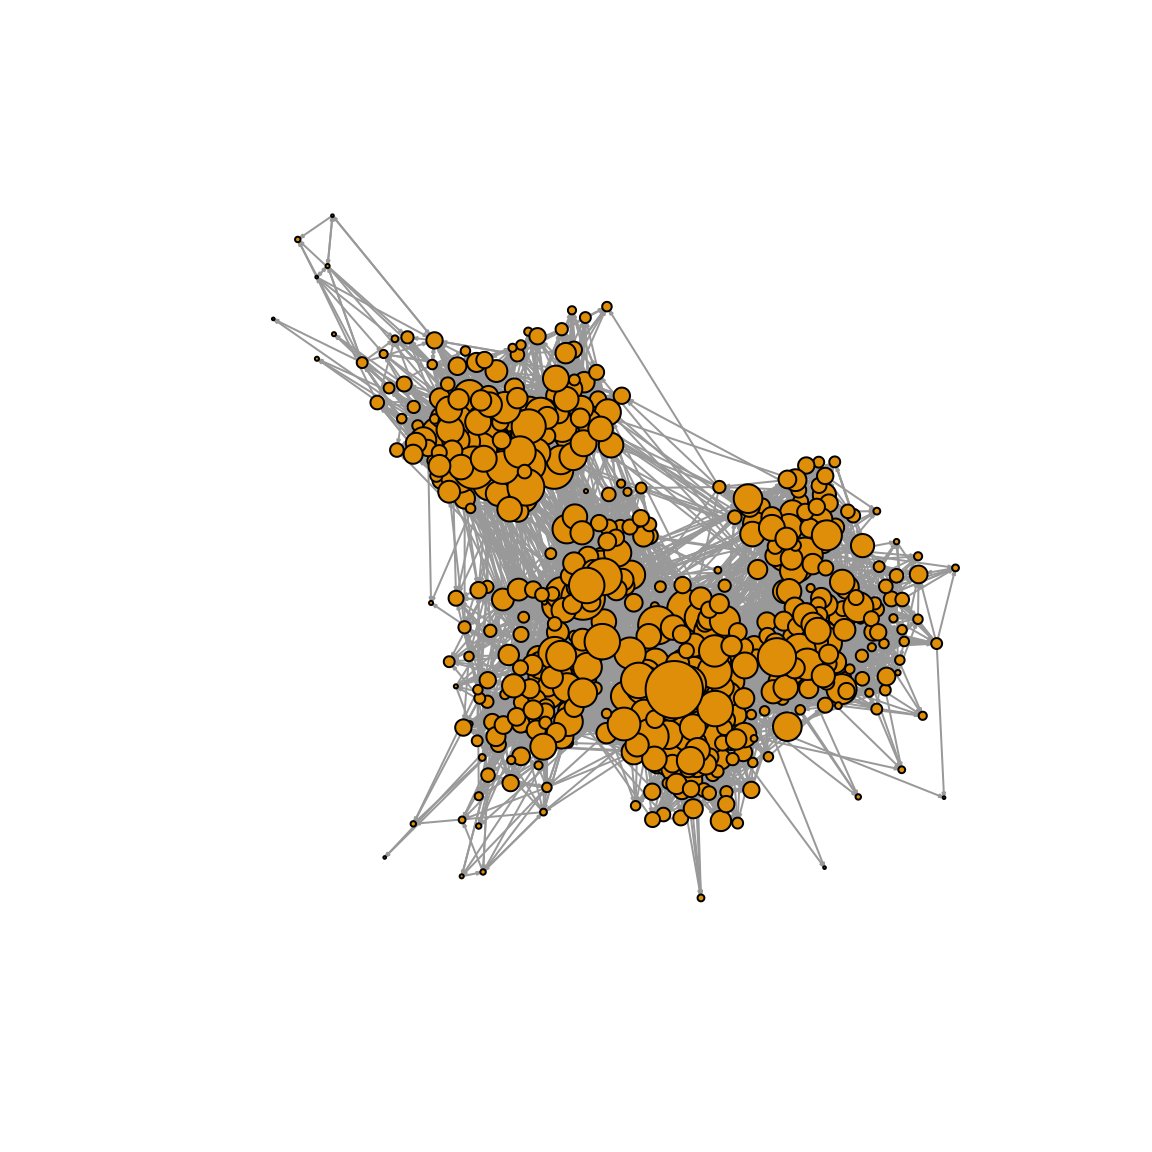
\includegraphics[keepaspectratio]{network_analyses_files/figure-latex/unnamed-chunk-3-1.pdf}}

\paragraph{Best friends}\label{best-friends}

\pandocbounded{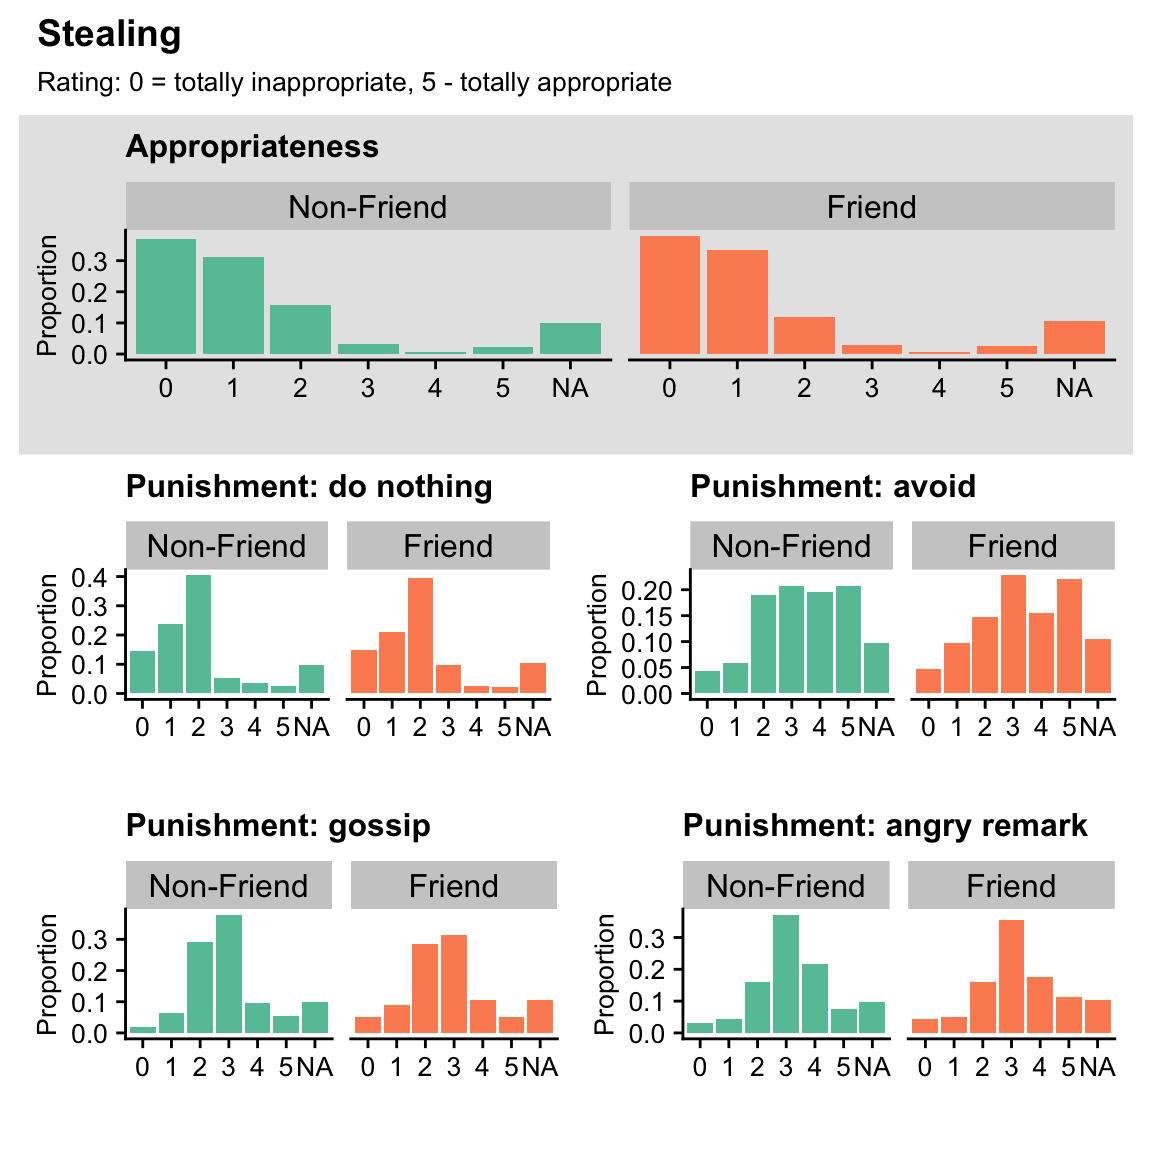
\includegraphics[keepaspectratio]{network_analyses_files/figure-latex/unnamed-chunk-4-1.pdf}}

\begin{longtable}[]{@{}lll@{}}
\caption{Network Summary}\tabularnewline
\toprule\noalign{}
Metric & GoodFriend & BestFriend \\
\midrule\noalign{}
\endfirsthead
\toprule\noalign{}
Metric & GoodFriend & BestFriend \\
\midrule\noalign{}
\endhead
\bottomrule\noalign{}
\endlastfoot
Average degree & 29.06 & 16.99 \\
Average path length (largest component) & 3.25 & 8.76 \\
Degree (min - max) & 2 - 134 & 1 - 89 \\
Degree SD & 15.6 & 11.91 \\
Density & 0.026 & 0.015 \\
Diameter (largest component) & 7 & 26 \\
Largest component size & 562 & 555 \\
Number of components & 1 & 1 \\
Number of edges & 8165 & 4714 \\
Number of nodes & 562 & 555 \\
Reciprocity & 0.315 & 0.473 \\
\end{longtable}

\subsubsection{Distribution of network
properties}\label{distribution-of-network-properties}

\begin{verbatim}
## [1] 8.043636
\end{verbatim}

\pandocbounded{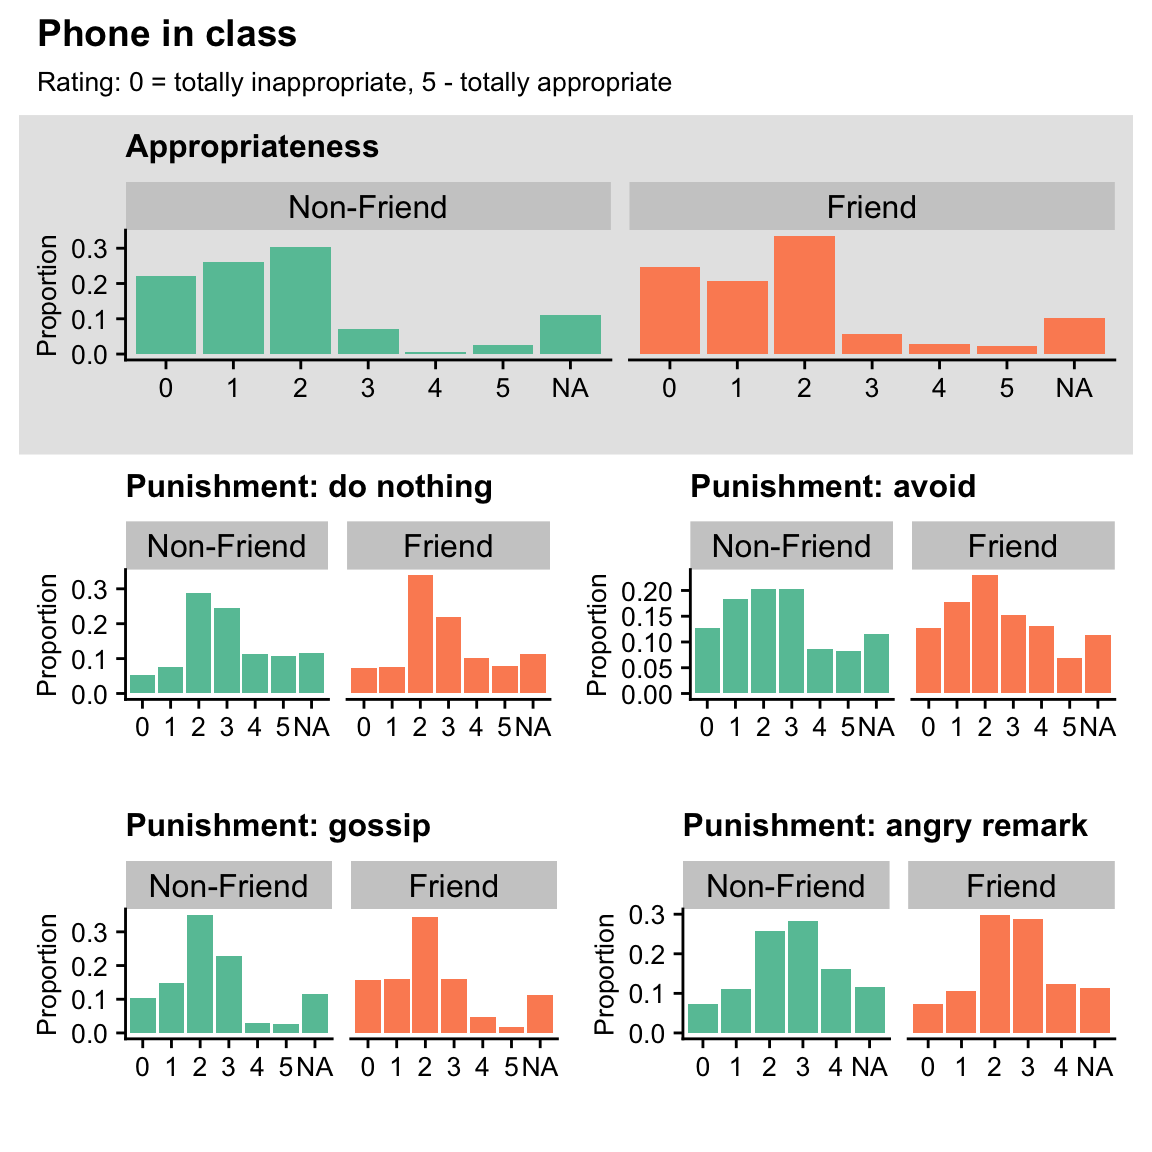
\includegraphics[keepaspectratio]{network_analyses_files/figure-latex/unnamed-chunk-5-1.pdf}}
\pandocbounded{\includegraphics[keepaspectratio]{network_analyses_files/figure-latex/unnamed-chunk-5-2.pdf}}
\pandocbounded{\includegraphics[keepaspectratio]{network_analyses_files/figure-latex/unnamed-chunk-5-3.pdf}}
\pandocbounded{\includegraphics[keepaspectratio]{network_analyses_files/figure-latex/unnamed-chunk-5-4.pdf}}
\pandocbounded{\includegraphics[keepaspectratio]{network_analyses_files/figure-latex/unnamed-chunk-5-5.pdf}}
\pandocbounded{\includegraphics[keepaspectratio]{network_analyses_files/figure-latex/unnamed-chunk-5-6.pdf}}
\pandocbounded{\includegraphics[keepaspectratio]{network_analyses_files/figure-latex/unnamed-chunk-5-7.pdf}}

\end{document}
